% #############################################################################
% This is Chapter 6
% !TEX root = ../main.tex
% #############################################################################
% Change the Name of the Chapter i the following line
\fancychapter{Sintax}
\cleardoublepage
% The following line allows to ref this chapter
\label{chap:sintax}

\section{Chapter 1}

\enquote{Cras gravida, diam sit amet rhoncus ornare, erat elit consectetuer erat, id egestas pede nibh eget odio.}

Pellentesque nibh felis, eleifend id, commodo in, interdum vitae, leo. 
 Praesent mauris \ac{SD} and \ac{HD} volutpat ligula eget enim \acp{WLAN} and 3G\slash 4G \acp{WWAN}.\todo[color=cyan!40, author=RC]{use of ACRONYM defined in file ``Thesis-MSc-Aconyms.tex''}


For example, the initial diameter (\gls{diam0}) of the tube corresponds to a surface area (\gls{surfarea}) of $122 \mu{m}^2$.

 
Please notice the use of automatic referencing to objects such as Figures, Tables, equations, Algorithms, sections of a document, etc. by using the command \verb:\Cref{ref}: as in this case pointing to \Cref{fig:cashed}.\ac{WLAN} is a acronym

\begin{figure}[htb]
\centering
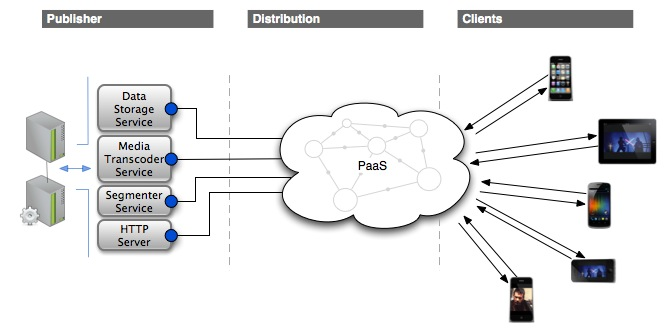
\includegraphics[width=0.9\textwidth]{./Images/cashed5}
\caption{Ecosystem}
\label{fig:cashed}
\end{figure}


\textcolor{violet}{You can use in-paragraph lists with this construct for: 
\begin{inparaenum}[(a)]
\item first case;
\item second case; and
\item third case,
\end{inparaenum}
making the text organized and fluid.}

Notice that \gls{maths} makes extensive use of \Glspl{formula}\todo[color=cyan!40, author=RC, fancyline]{example of use of Glossaries}{} which are particularly well rendered in documents produced with \gls{LaTeX}.

% #############################################################################

\section{Chapter 2}

\begin{table}[htb]
\centering
\normalsize
{\footnotesize
    \caption{Streaming Technologies Comparison}
    \label{tab:streamingtech}
    \begin{tabular}{ | c | c | c | c |}
    \hline
    & Dynamic & Smooth & HLS\\
    & Streaming & Streaming & \\ \hline \hline

    Streaming Protocol & RTMP & HTTP & HTTP \\
    %\textbf{Protocol} & & & \\ 
    \hline
    
    Video Codec & H.264, VP6 & H.264 & H.264 \\ 
    %\textbf{Codec} & &  & \\ 
    \hline
    
    Audio Codec & AAC, MP3 & WMA, AAC & AAC, MP3  \\
    %\textbf{Codec} & & & \\ 
    \hline
    
    Container Format & MP4, FLV, & MP4 & MPEG2-TS \\
    %\textbf{Format} & F4V & & \\ 
    \hline
    
     iOS & NO & YES & YES \\ \hline
     
    Android & NO & YES & YES \\ \hline
    
    \end{tabular}
    }
\end{table} 

use of a Spreadsheet-like table producing calculations by columns and by lines
(observe the code)

\begin{table}[htb]
\centering
    \caption{A nice Spreadsheet using package ``spreadtab''. Notice the calculations.}
    \label{tab:spreadtb}
\begin{spreadtab}{{tabular}{rr|r}} 
22       & 54       & a1+b1 \\
43       & 65       & a2+b2 \\ 
49       & 37       & a3+b3 \\
\hline
a1+a2+a3 & b1+b2+b3 & a4+b4
\end{spreadtab}
\end{table}

{\Cref{tab:comp_arch} is automatically compressed to fit text width. You can use \url{https://www.tablesgenerator.com} to produce these tables, and then copy the \LaTeX\space code generated to paste in the document.}

\begin{table}[ht]
\centering
\caption{Comparison between today's and target Architectures of Telcos}
\label{tab:comp_arch}
\resizebox{\textwidth}{!}{%
\begin{tabular}{|
>{\columncolor[HTML]{ECF4FF}}l |l|
>{\columncolor[HTML]{E2FFC9}}l |l|}
\hline
\multicolumn{2}{|c|}{\cellcolor[HTML]{ECF4FF}Today}                                                                                                             & \multicolumn{2}{c|}{\cellcolor[HTML]{E2FFC9}Target}                                                                                  \\ \hline
Rigid     & \begin{tabular}[c]{@{}l@{}}Each evolutionary requirement involves \\ development of multiple components, \\ interfaces, platforms,etc.\end{tabular} & Flexible       & \begin{tabular}[c]{@{}l@{}}It is possible to modify or add new\\ functionalities rapidly.\end{tabular}              \\ \hline
Slow      & \begin{tabular}[c]{@{}l@{}}Development of a new application takes \\ months or years.\end{tabular}                                                  & Fast           & \begin{tabular}[c]{@{}l@{}}Development of a new application takes \\ weeks instead of months or years.\end{tabular} \\ \hline
Closed    & \begin{tabular}[c]{@{}l@{}}Limited integration with external\\ environments.\end{tabular}                                                           & Open           & \begin{tabular}[c]{@{}l@{}}It is simple to integrate internal,\\ applications with external entities.\end{tabular}  \\ \hline
Complex   & \begin{tabular}[c]{@{}l@{}}Heterogeneous technologies, obsolescence, \\ lack,of standards, high redundancy.\end{tabular}                            & Standardised   & Use of homogeneous architectural models.                                                                            \\ \hline
Expensive & \begin{tabular}[c]{@{}l@{}}High Capex (for new service development) \\ and,high,Opex (to ensure running of IT).\end{tabular}                        & Cost-Effective & Capex and Opex are optimised.                                                                                       \\ \hline
\end{tabular}
}
\end{table}

% #############################################################################

\section{Chapter 3}

\textcolor{violet}{Example of a Flowchart for a system, in \Cref{fig:flowchart}, created with \url{https://app.diagrams.net} and then exported as ``PDF'' crop format (a true vector image that can be scaled to no end, with no pixels or distortion).}

\begin{figure}[ht]
\centering
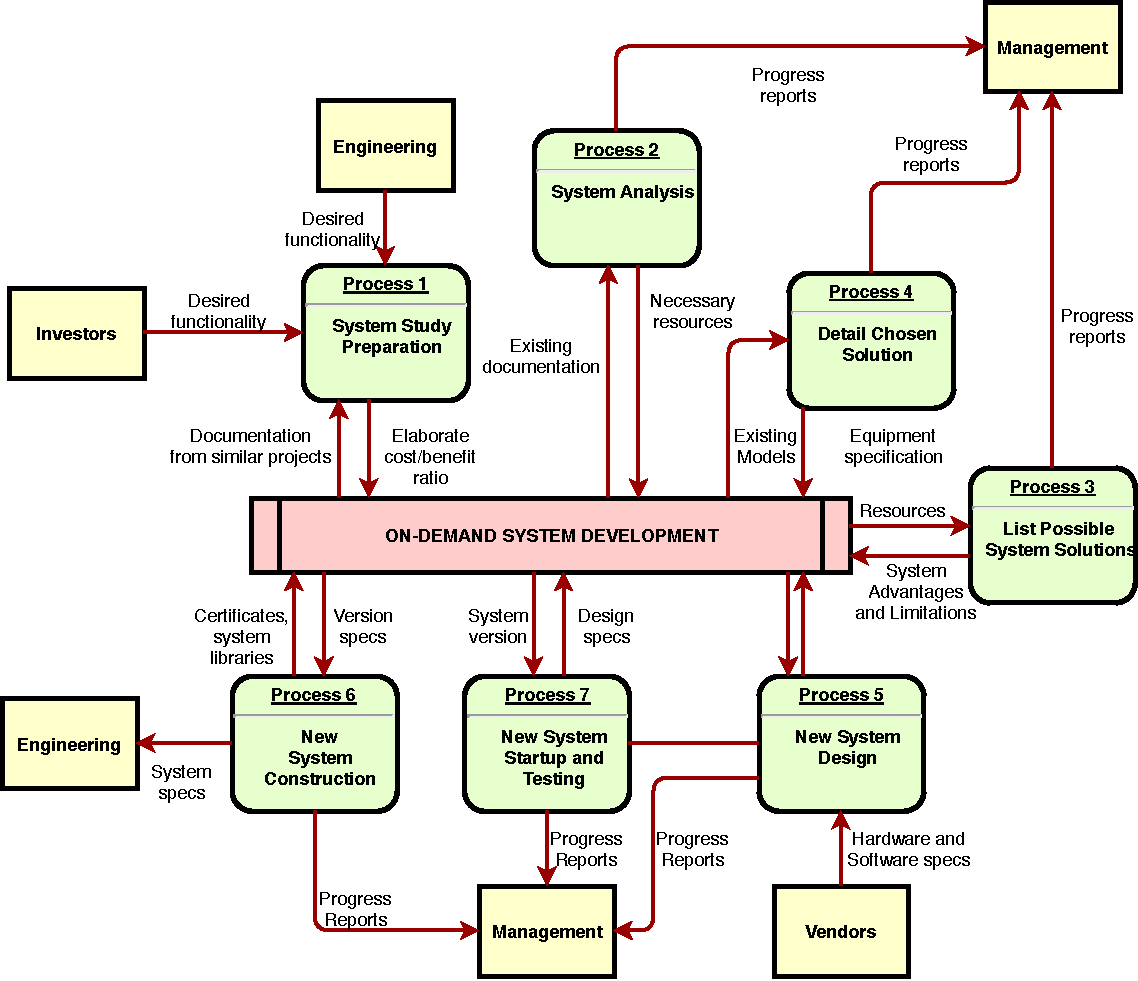
\includegraphics[width=1.0\textwidth]{./Images/Flowchart_from_draw-io.pdf}
\caption{System Processes}
\label{fig:flowchart}
\end{figure}

\textcolor{violet}{And here another diagram of a network (\Cref{fig:network}) created with \url{https://app.diagrams.net} and then exported as ``PDF'' crop format.}

\begin{figure}[ht]
\centering
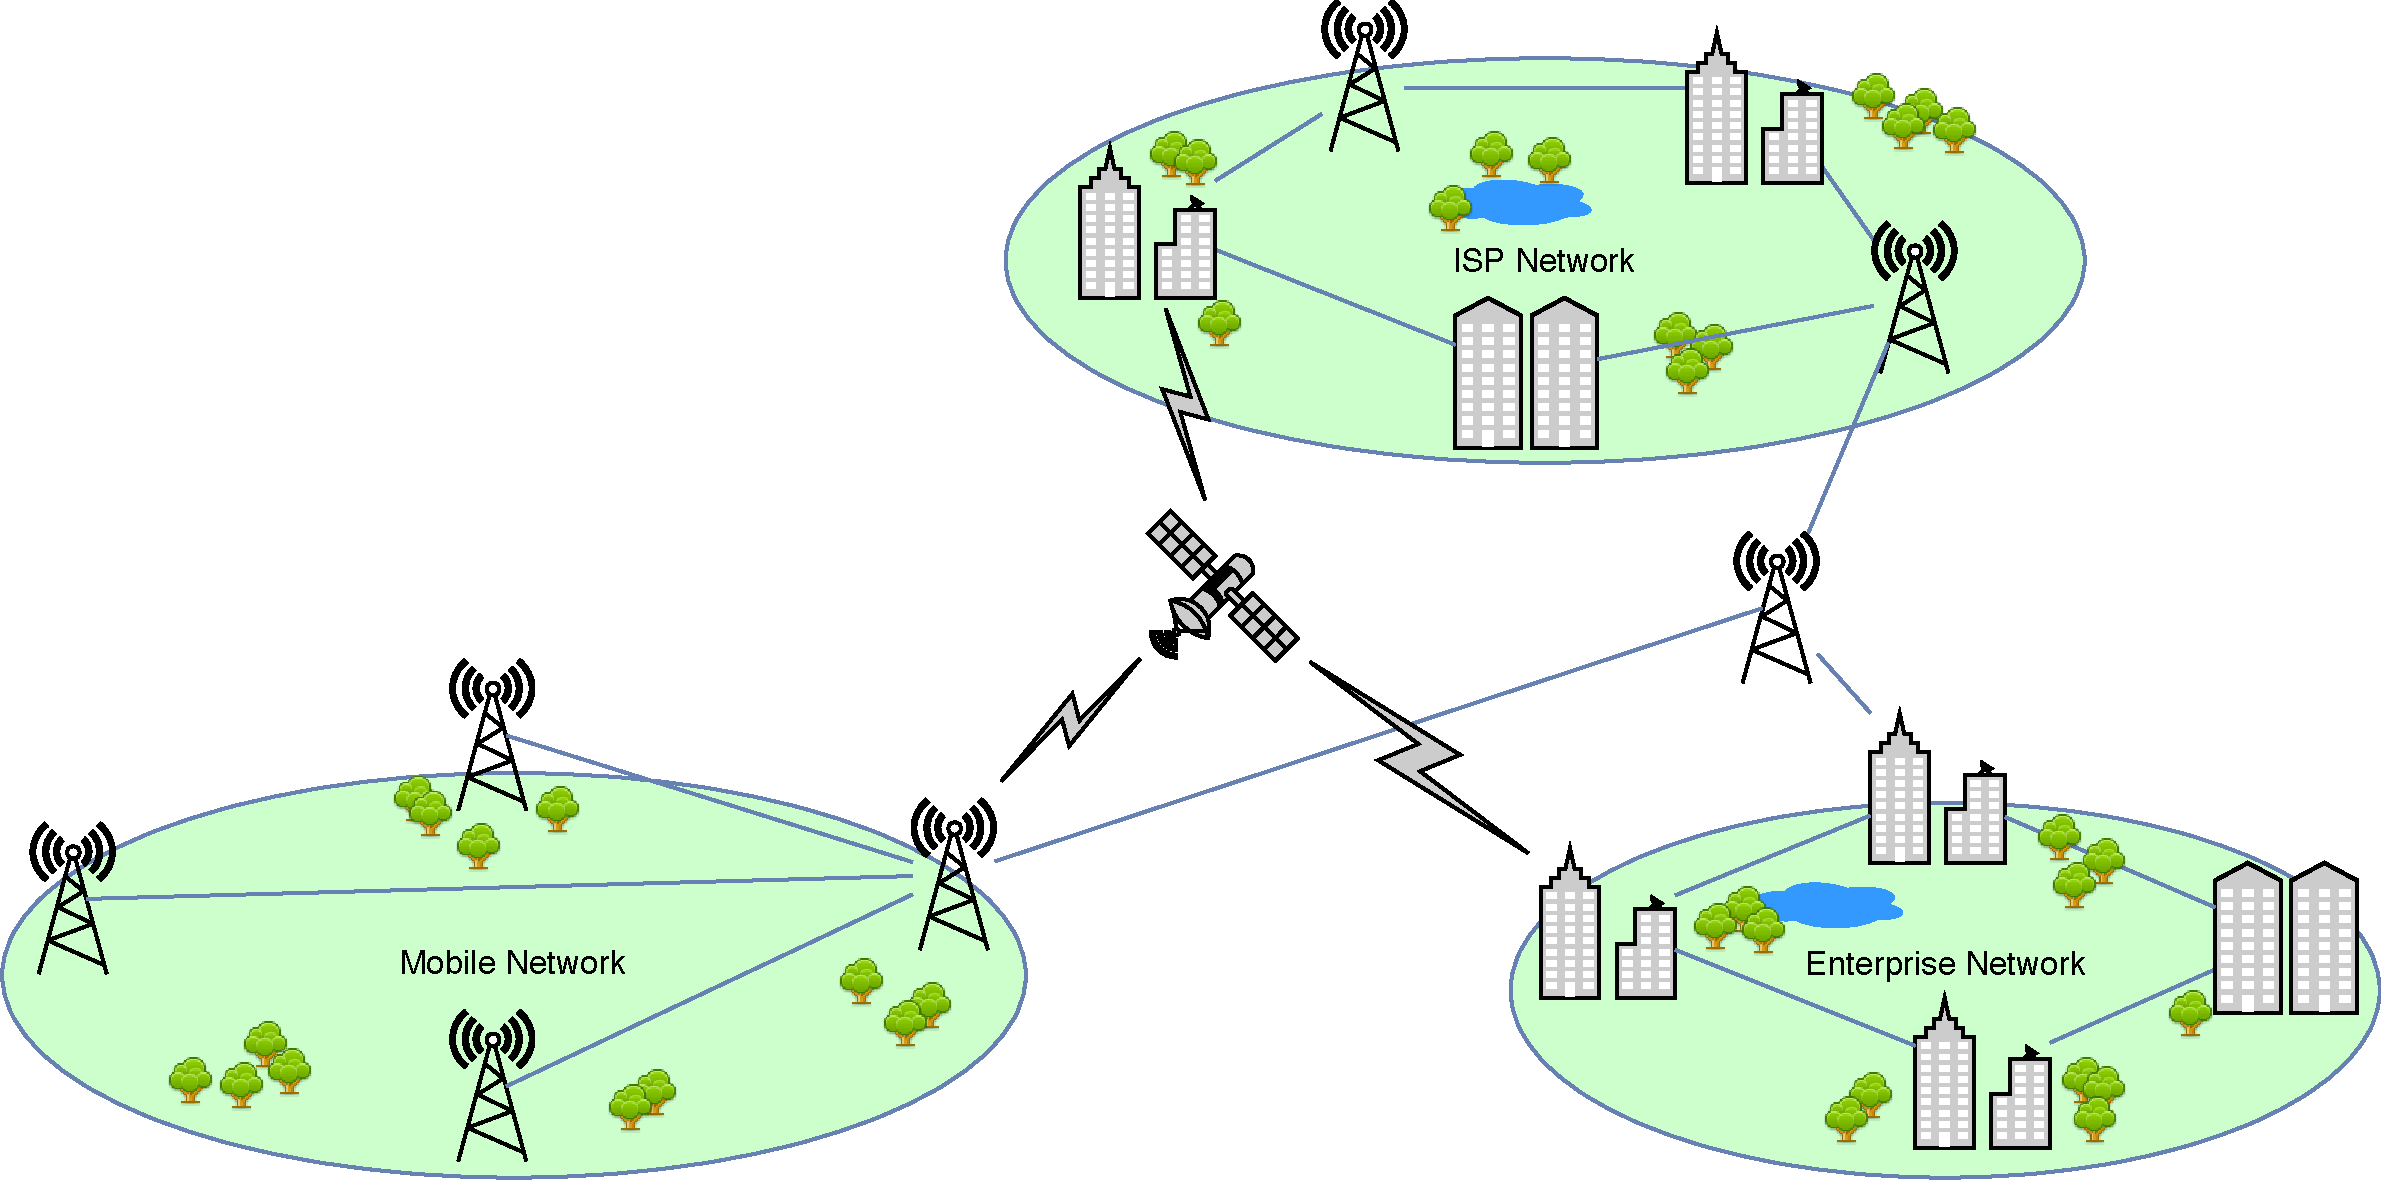
\includegraphics[width=1.0\textwidth]{./Images/Network_from_draw-io.pdf}
\caption{Network Diagram}
\label{fig:network}
\end{figure}

\begin{description}
	\item[\textbf{Web-streaming:}]
	The client application should support streaming media using \ac{HTTP} protocols.
	\item[\textbf{Multi-source streaming:}]
	The client application should support multi-source streaming media, i.e., ``simultaneous'' streaming of media content components from a network, supported\slash complemented by \ac{CDN}\slash \ac{CC} services. 
	\item[\textbf{Support content Metadata Description:}]
	The client application should support content metadata description in a format similar or compliant with MPEG \ac{DASH} \cite{ISO/IEC:2012fk}. 
	\item[\textbf{Scalable and Adaptive Media Contents:}]
	The system should support on-demand streaming of scalable and adaptive contents based on \ac{SVC}.
	\item[\textbf{Heterogenous End-User Devices:}]
	The client application should be compatible with current and future generations of end-user devices form factors, irrespective of their performance, screen size and resolution.
	\item[\textbf{Access Network independency:}] 
	The solution should provide the expected service over different types of access networks supported by the end-user devices, such as Wireless \acp{LAN} (IEEE 802.11) or cellular data networks such as \ac{GPRS}, \ac{UMTS}, \ac{LTE}, etc.
\end{description}

\Cref{mpd}\todo[color=cyan!40, author=RC, fancyline]{A listing for XML code, with syntax highlighting}{}.

\begin{minipage}[c]{0.95\textwidth}
\begin{center}
\begin{spacing}{0.5}
\begin{lstlisting}[frame=lines,style=XML,caption={Example of a MPD file.},label=mpd]
<?xml version="1.0" encoding="UTF-8"?>
<StreamInfo version="2.0">
    <Clip duration="PT01M0.00S">
        <BaseURL>videos/</BaseURL>
        <Description>svc_1</Description>
        <Representation mimeType="video/SVC" codecs="svc" frameRate="30.00" bandwidth="401.90"
            width="176" height="144" id="L0">
            <BaseURL>svc_1/</BaseURL>
            <SegmentInfo from="0" to="11" duration="PT5.00S">
                <BaseURL>svc_1-L0-</BaseURL>
            </SegmentInfo>
        </Representation>
        <Representation mimeType="video/SVC" codecs="svc" frameRate="30.00" bandwidth="1322.60"
            width="352" height="288" id="L1">
            <BaseURL>svc_1/</BaseURL>
            <SegmentInfo from="0" to="11" duration="PT5.00S">
                <BaseURL>svc_1-L1-</BaseURL>
            </SegmentInfo>
        </Representation>
    </Clip>
</StreamInfo>
\end{lstlisting}
\end{spacing}
\end{center}
\end{minipage}

% #############################################################################

\section{Chapter 4}

\begin{itemize}
\item{Technology Research and Related Works}
\item{Requirements Gathering and Study}
\item{Design of the Architecture}
\item{Implementation Process}
\item{Testing and Functional Validation}
\end{itemize}

\Cref{time_control_algorithm}\todo[color=cyan!40, author=RC, fancyline]{Notice the reference to the Algorithm construct}{}

\begin{algorithm}[ht]
\DontPrintSemicolon
\Begin{
$nextBitrate \longleftarrow nextDownloadLevel$\;
$nextBitrate \longleftarrow GetNextBitrate()$\;
$cpuLoad \longleftarrow GetCpuLoad()$\;
$bitrateDelta \longleftarrow getBitrateDelta(currentBitrate, nextBitrate)$\;
\BlankLine
\If{$bitrateDelta > maxThreshold$}{
     $SetBitrate(nextBitrate)$\;
   }
\BlankLine
  \If{$minThreshold < bitrateDelta < maxThreshold$ {\bf and} $numAttemps < 2$}{ 
       $numAttemps \longleftarrow numAttemps + 1$\;
       }{
       \uElseIf{$minThreshold < bitrateDelta < maxThreshold$ {\bf and} $numAttemps = 2$}{
       $numAttemps \longleftarrow 0$\;
       }
       \Else{$SetBitrate(nextBitrate)$}
      }
  \If{$0 < bitrateDelta < minThreshold$ {\bf and} $numAttemps < 3$}{
       $numAttemps \longleftarrow numAttemps + 1$\;
       }{
       \uElseIf{$0 < bitrateDelta < minThreshold$ {\bf and} $numAttemps = 3$}{
       $SetBitrate(nextBitrate)$\;
       }
       }
}
\caption{Time Control Strategy}
\label{time_control_algorithm}
\end{algorithm}

\begin{minipage}[c]{1.0\textwidth}
%\begin{center}
\centering
\begin{lstlisting}[language = C++, numbers = none, escapechar = !,
    basicstyle = \ttfamily\bfseries, linewidth = .6\linewidth, frame=tb, caption={A listing with a Tikz picture overlayed}, captionpos=b, label=tikzlist] 
 int!
   \tikz[remember picture] \node [] (a) {};
 !puissance!
   \tikz[remember picture] \node [] (b) {};
 !(int x,!
   \tikz[remember picture] \node [] (c){};
 !int n) { 

     int i, p = 1; !\tikz[remember picture] \node [] (d){};!           

     for (i = 1; i <= n; i++) 
       p = p * x; !\tikz[remember picture] \node [inner xsep = 40pt] (e){};! 

     return p; !
       \tikz[remember picture] \node [] (f){};!  
 }
\end{lstlisting}

\begin{tikzpicture}[remember picture, overlay,
    every edge/.append style = { ->, thick, >=stealth,
                                  darkgray, dashed, line width = 1pt },
    every node/.append style = { align = center, minimum height = 10pt,
                                 font = \bfseries, fill= green!20},
                  text width = 2.5cm ]
  \node [above left = .75cm and -.75 cm of a,text width = 2.2cm]
                             (A) {return value type};
  \node [right = 0.25cm of A, text width = 1.9cm]
                             (B) {function name};
  \node [right = 0.5cm of B] (C) {list of formal parameters};
  \node [right = 4.cm of d]  (D) {local variables declaration};
  \node [right = 2.cm of e]  (E) {instructions};
  \node [right = 5.cm of f]  (F) {instruction \texttt{\bfseries return}};  
  \draw (A.south) + (0, 0) coordinate(x1) edge (x1|-a.north);
  \draw (B.south) + (0, 0) coordinate(x2) edge (x2|-b.north);
  \draw (C.south) + (0, 0) coordinate(x3) edge (x3|-c.north);
  \draw (D.west) edge (d.east) ;
  \draw (E.west) edge (e.east) ;  
  \draw (F.west) edge (f.east) ;
\end{tikzpicture}
%\end{center}
\end{minipage}

\textcolor{violet}{And here another method (\Cref{tikzlist}) for mixing (overlay) a picture with a listing of code.}

\Cref{fig:ui_playout,fig:ui_loading}\todo[color=cyan!40, author=RC, fancyline]{A figure with Subfigures}{}

\begin{figure}[htbp]
	\centering
	\subfigure[Media Loading Window]{\label{fig:ui_loading} 		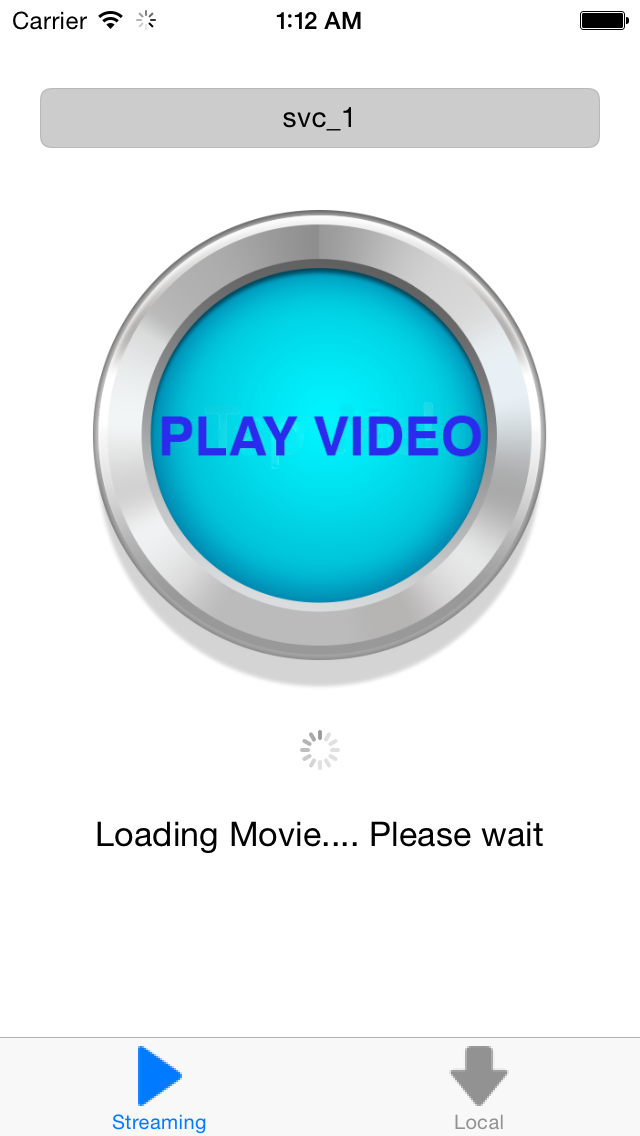
\includegraphics[width=0.3\textwidth]{./Images/ui_loading}} \qquad
	\subfigure[Play-out Session UI]{\label{fig:ui_playout}
		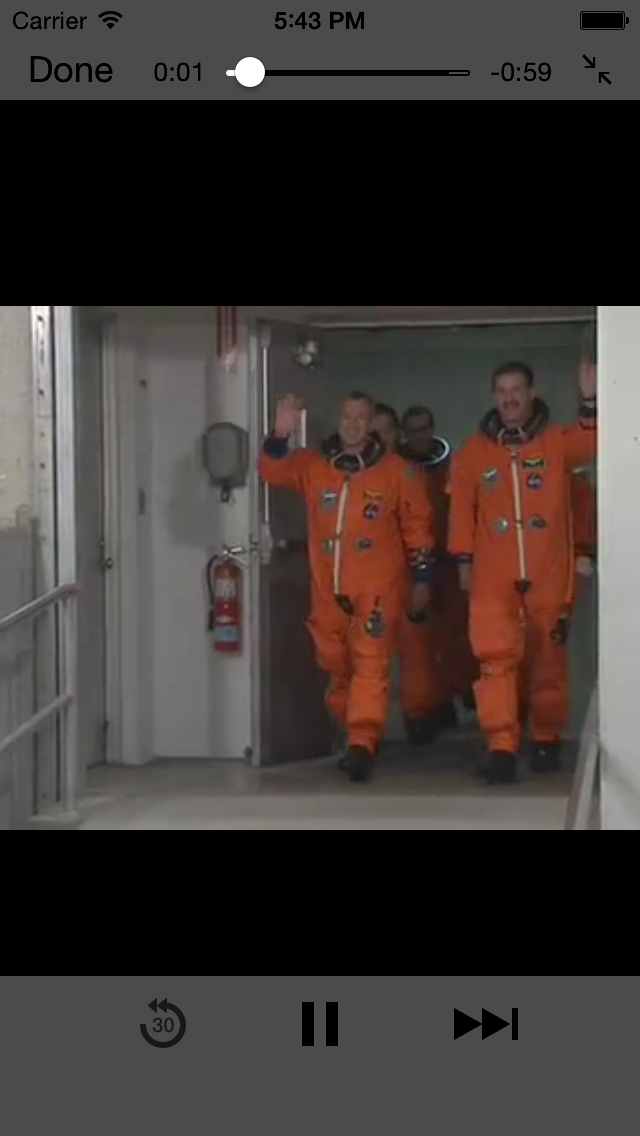
\includegraphics[width=0.3\textwidth]{./Images/ui_playout}}
	\caption{Complete User Interface}
	\label{fig:user_interface}
\end{figure}

% #############################################################################

\section{Chapter 5}

\begin{figure}[ht]
\centering
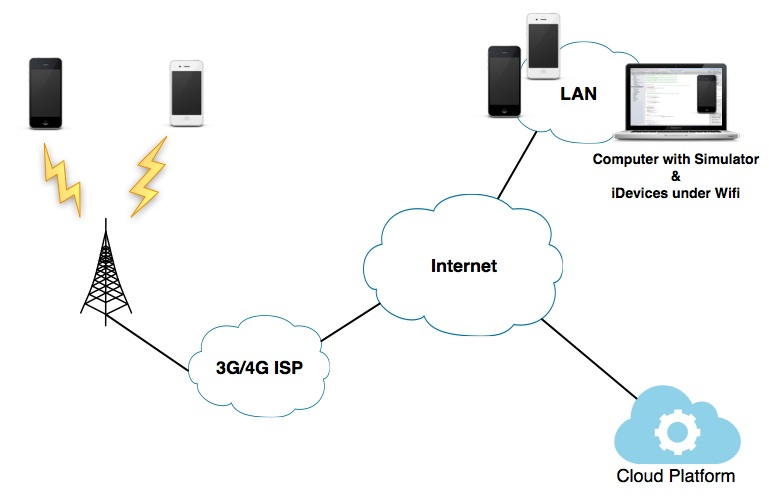
\includegraphics[width=0.8\textwidth]{./Images/test_env}
\caption{Test Environment}
\label{fig:test_env}
\end{figure}

\begin{table}[htb]
\centering
\normalsize
    \caption{Network Link Conditioner Profiles}
    \label{tab:network_profiles}
{\footnotesize
    \begin{tabular}{ | c | c | c | c | }
    \hline 
    \textbf{Network Profile}	& \textbf{Bandwidth} & \textbf{Packets Droped} & \textbf{Delay}\\ \hline \hline
    Wifi  & 40 mbps  &  0\%  &   1 ms \\ \hline
    3G  & 780 kbps  &  0\%  &   100 ms \\ \hline 
    Edge  & 240 kbps  &  0\%  &   400 ms \\ \hline
    \end{tabular}
    }
\end{table}

\begin{description}
  \item[$N_j$] Is the number of times peer $j$ has been optimistically unchoked.
  \item[$n_j$] Among the $N_j$ unchokes, the number of times that peer $j$ responded with unchoke or supplied segments to peer $p$.
  \item[$C_{r[j]}$] The cooperation ratio of peer $j$. If peer $j$ never supplied peer $p$, the information of $C_{r[j]}$ may not be available.
  \item[$C_{r (max)}$] The maximum cooperation ratio of peer $p$’s neighbors, i.e., $C_{r (max)} = max(C_r)$.
\end{description}

\begin{equation}
\label{unchoke_gain}
 G_j =
  \begin{dcases}
    \frac{n_j C_{r[j]}}{N_j} &\quad \text{if } n_j > 0\\
    \frac{C_{r (max)}}{N_j + 1} &\quad \text{if } n_j = 0
  \end{dcases}
\end{equation}

$C_{r (max)}$ or $j$ or $N_j = 0$ or $G_j = C_{r (max)}$.

Both \Cref{fig:tx_layer_4,fig:tx_layer_5}

\begin{figure}[ht]
%\centering
       \subfigure[Adaptation System Test 4]{\label{fig:tx_layer_4}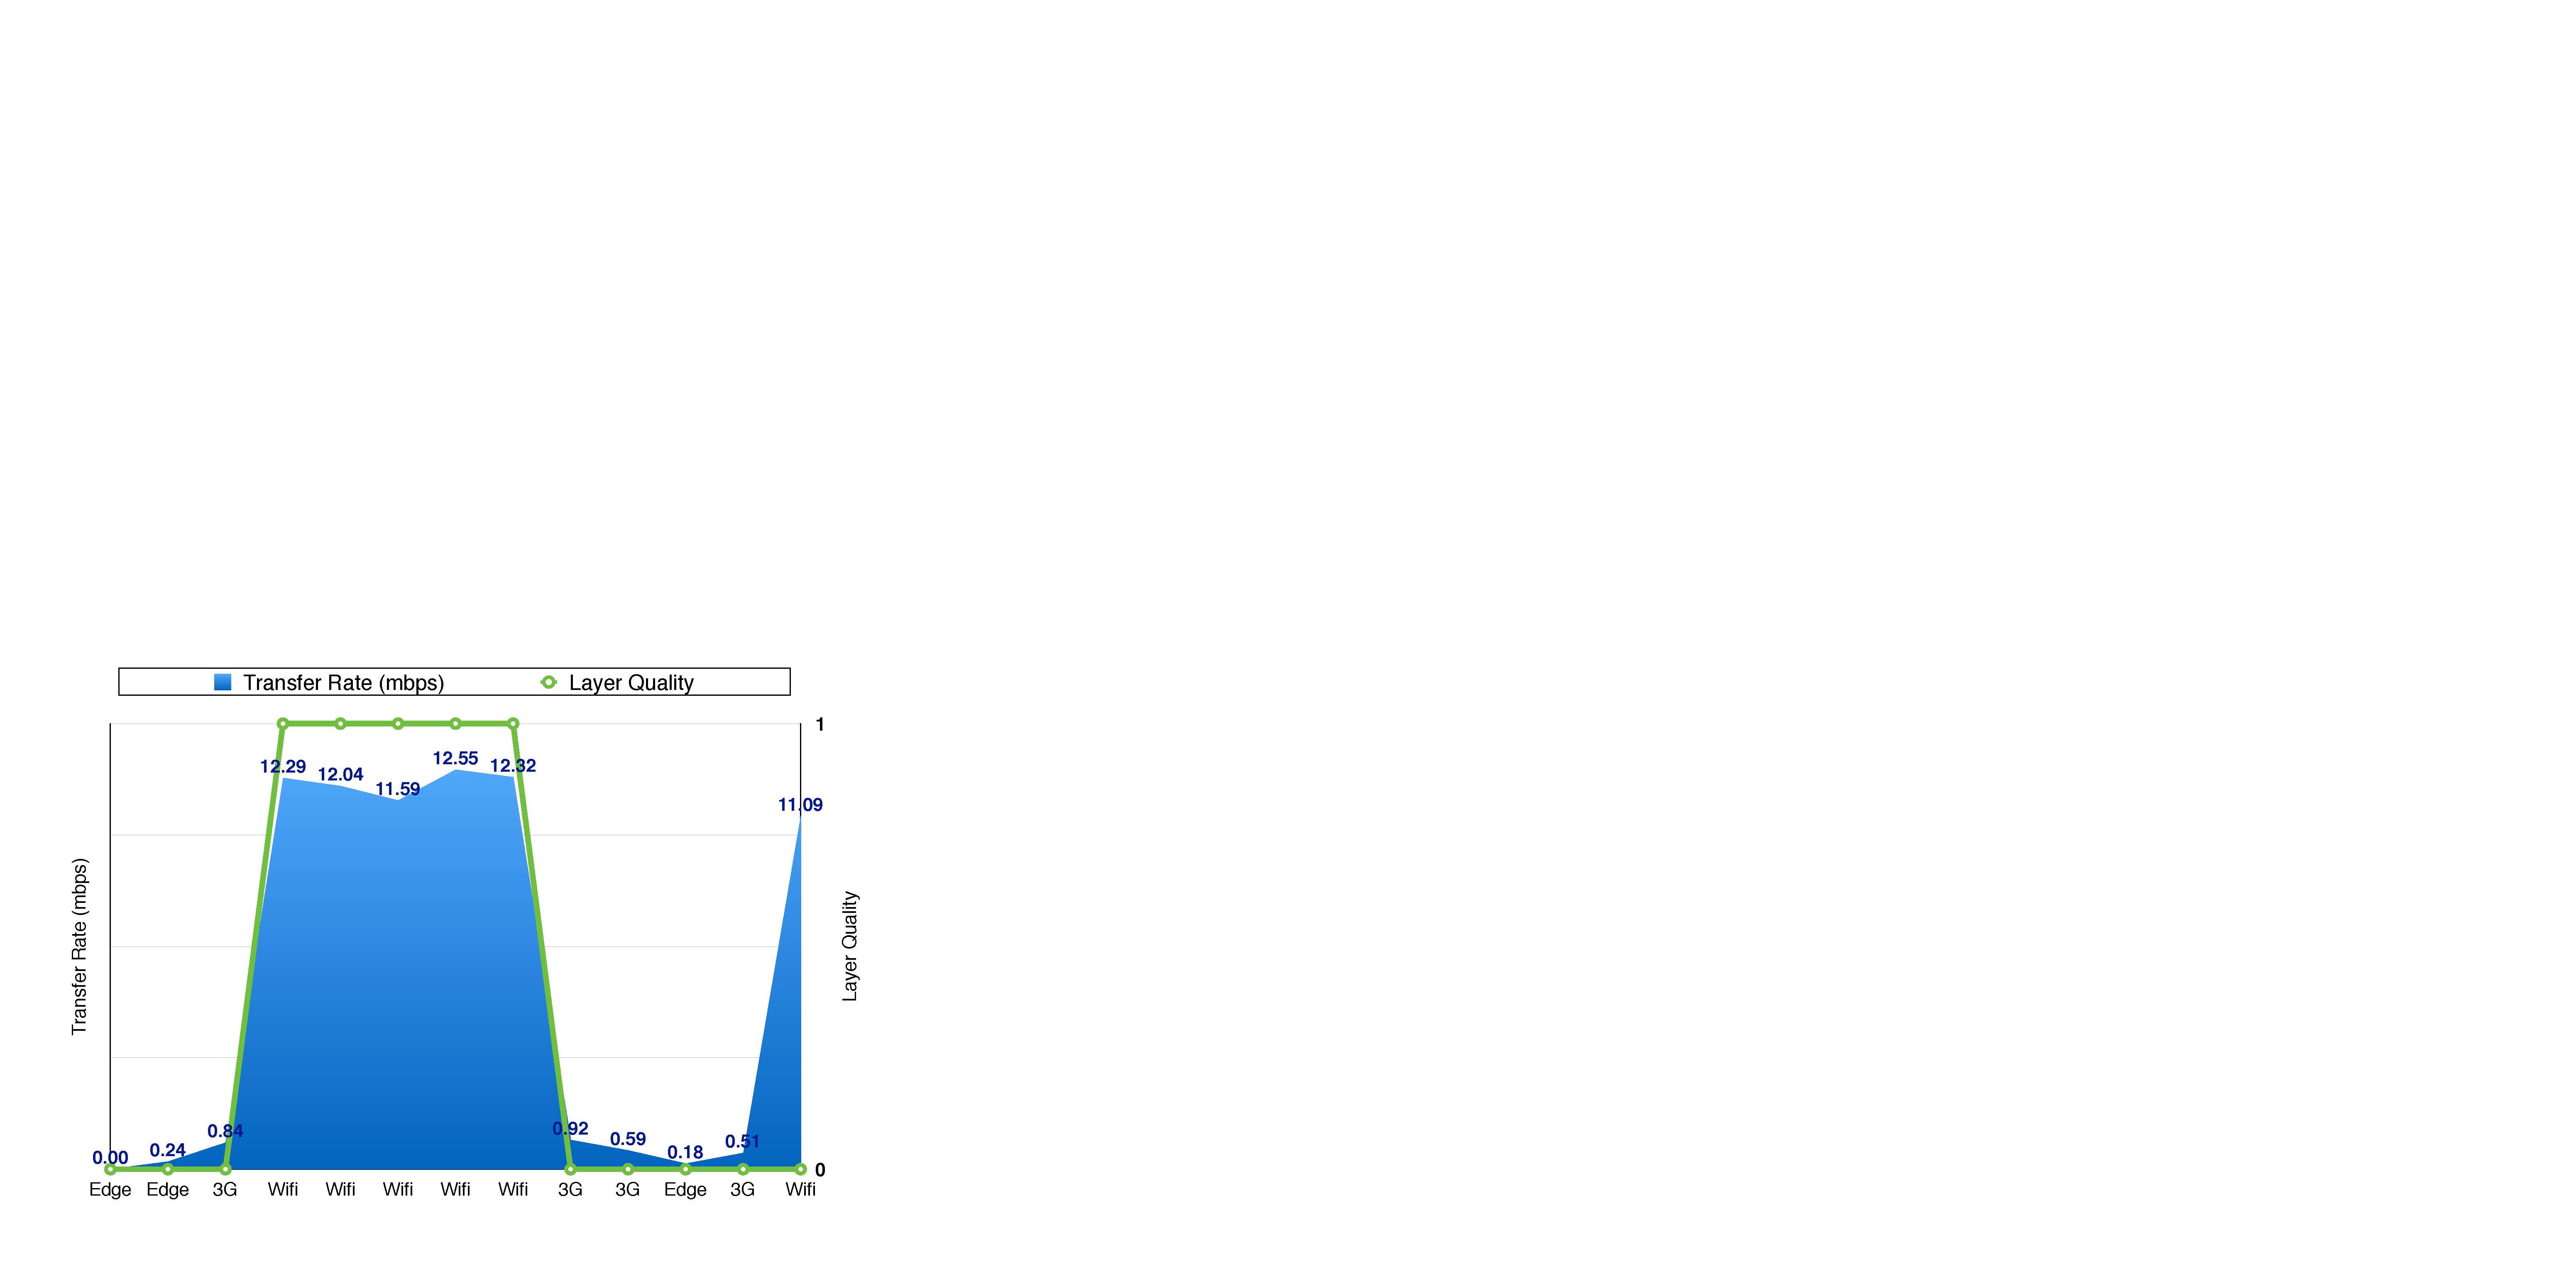
\includegraphics[width=0.5\textwidth]{./Images/tx_layer_4}}  
   %    \centering 
       \subfigure[Adaptation System Test 5]{\label{fig:tx_layer_5}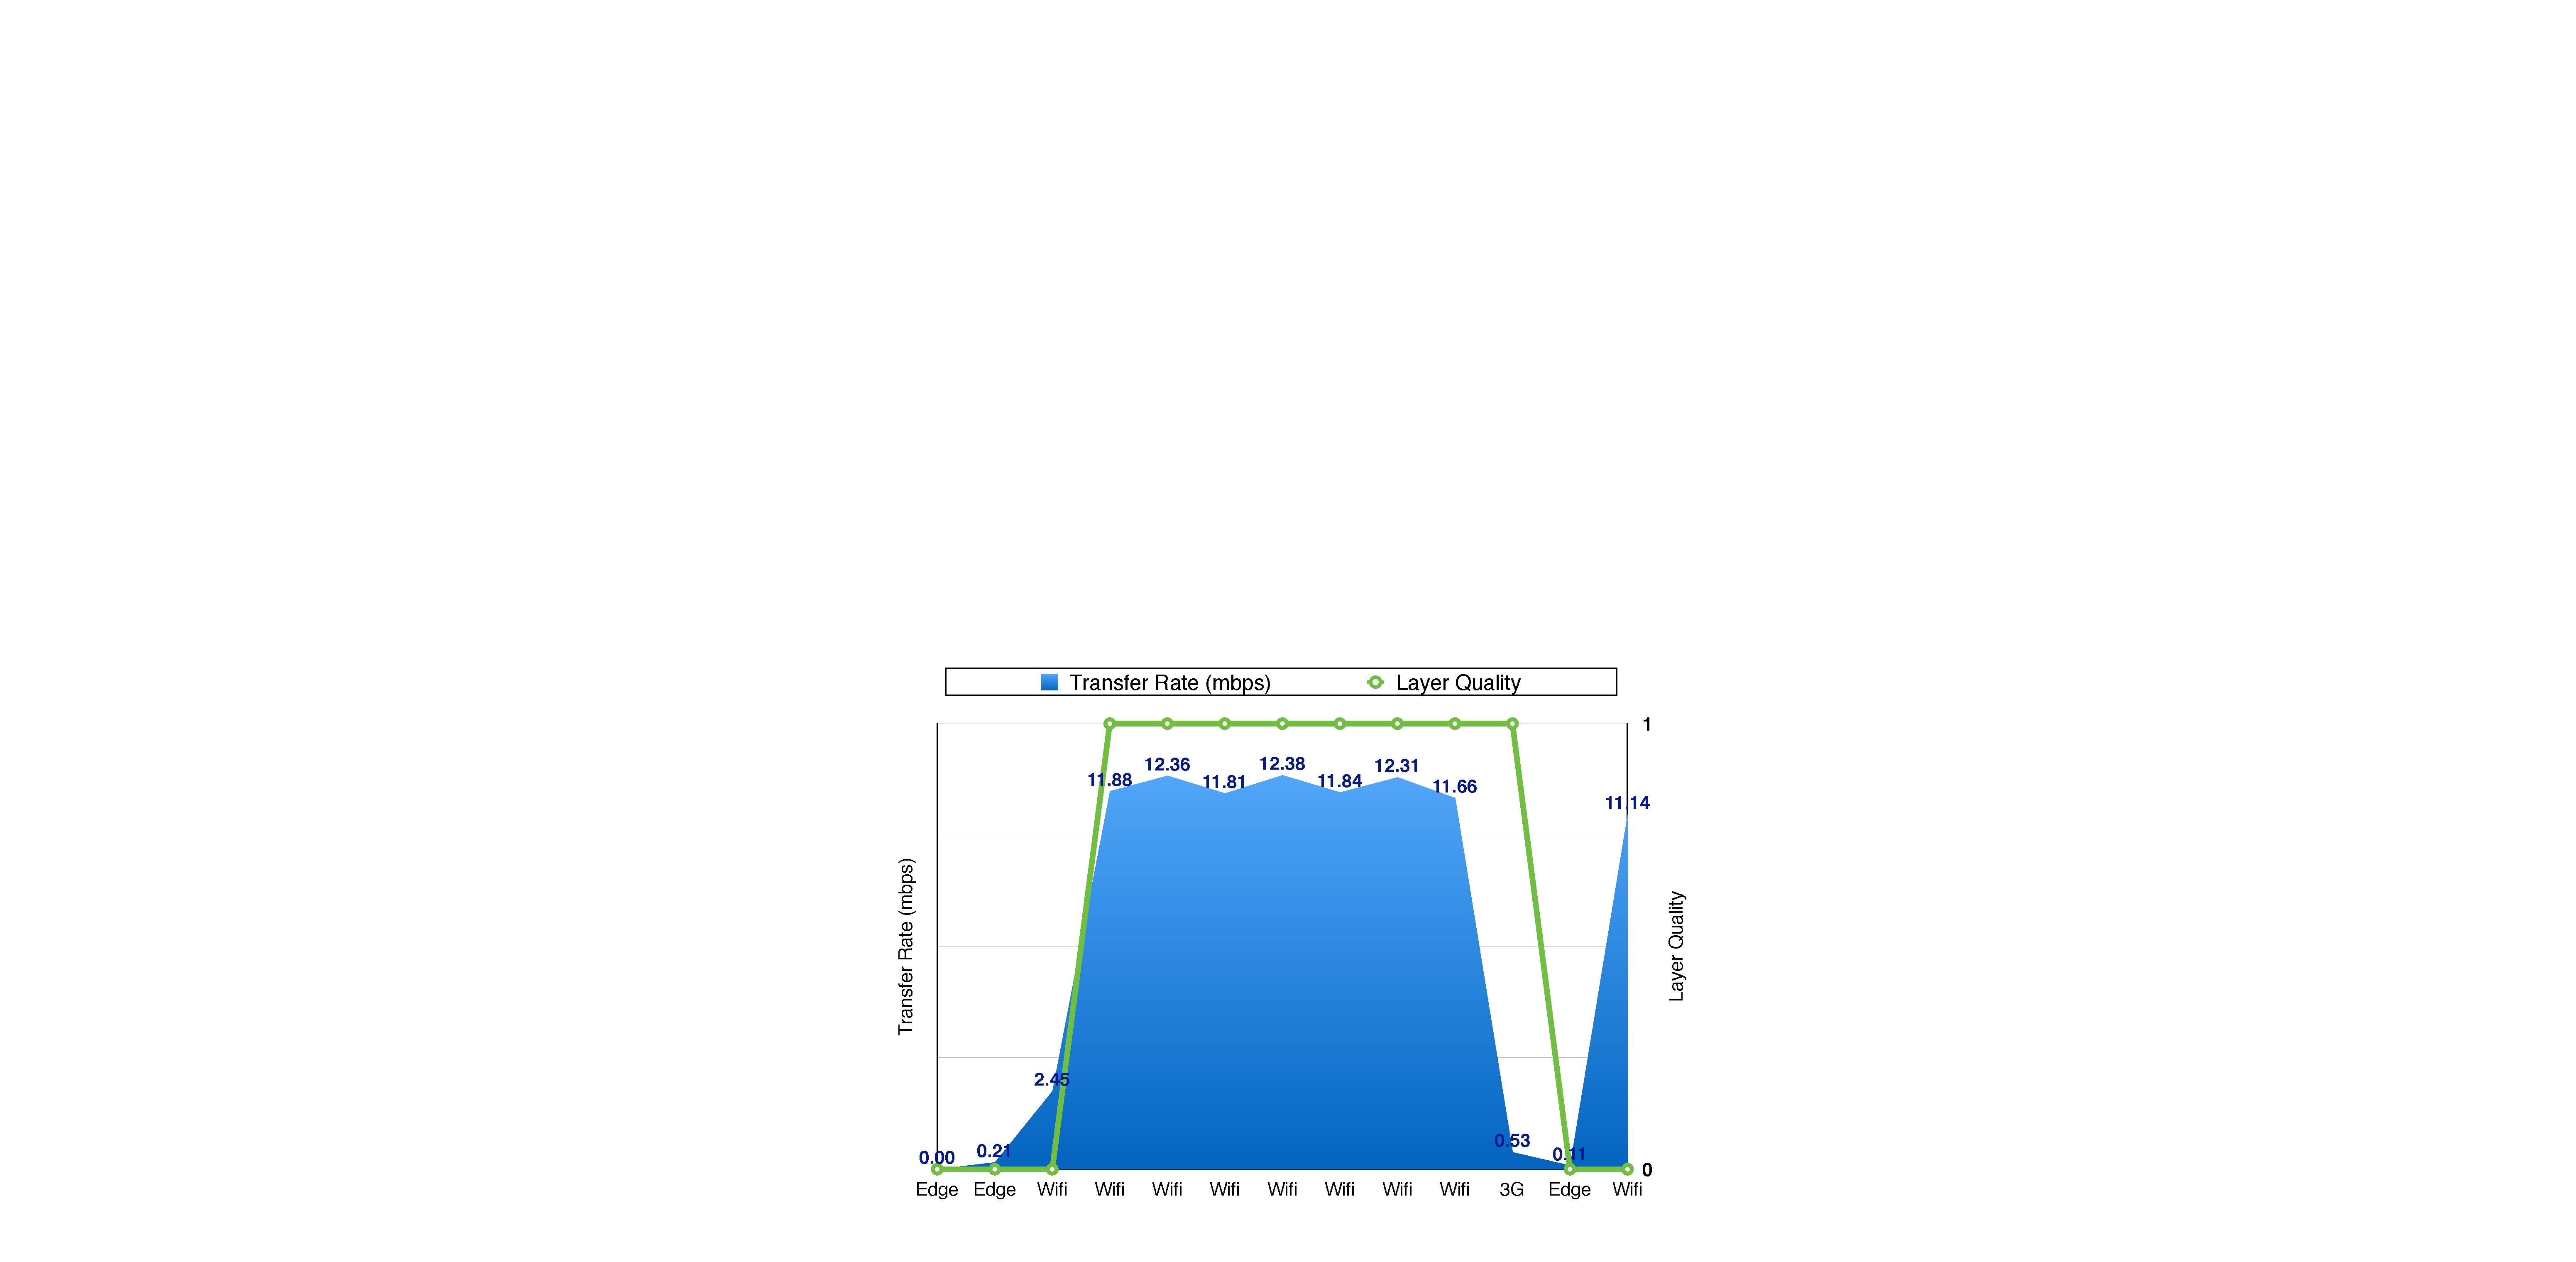
\includegraphics[width=0.5\textwidth]{./Images/tx_layer_5}}   
        \caption{Adaptation System Behavior Test}
        \label{fig:fig:adapt_behave_2}
\end{figure}
% #############################################################################

\section{Chapter 6}

% #############################################################################